\pdfoutput=1
\newcommand{\online}{0}
\newcommand{\classstyle}{1}
\documentclass[12pt]{article}
\usepackage[utf8]{inputenc} 
\usepackage{fullpage}
\usepackage{times}
\usepackage[normalem]{ulem}
\usepackage{fancyhdr,graphicx,amsmath,amssymb, mathtools, scrextend, titlesec, enumitem}
\setlength{\headheight}{14.49998pt}
\usepackage{bm}
\usepackage{tcolorbox}
\usepackage{amsthm}
\usepackage{mathrsfs} 
\usepackage{multicol} 
\usepackage[acronym,nomain,nonumberlist]{glossaries}


\makeglossaries

\usepackage{siunitx}
\setlist[itemize]{itemsep=0pt, parsep=0pt, topsep=0pt, partopsep=0pt, left=0pt}


%cross and mark
\usepackage{bbding}

% package subfigure
\usepackage{caption}
\usepackage{subcaption}

% tikz
\usepackage{tikz}
\newcommand{\tikzmark}[1]{\tikz[baseline,remember picture] \coordinate (#1) {};}
%line numbering
\usepackage{lineno}
\linenumbers
% \usepackage[dvipdfmx]{graphicx} 
% \usepackage{bmpsize}
\usepackage{booktabs}
\usepackage{multirow}


\usepackage{amsfonts}
\numberwithin{equation}{section}
\ifnum\classstyle=3
\else
\newtheorem{theorem}{Theorem}[section]
\newtheorem{definition}{Definition}[section]
\newtheorem{corollary}{Corollary}[section]
\newtheorem{lemma}{Lemma}[section]
\newtheorem{proposition}{Proposition}[section]
\newtheorem{remark}{Remark}[section]
\fi
\newtheorem{problem}{Problem}[section]
%\theoremstyle{definition}
\newtheorem{example}{Example}[section]
\newtheorem{assumption}{Assumption}[section]
\newtheorem{conjecture}{Conjecture}[section]

\ifnum\classstyle=3
\else
\usepackage[hypertexnames=false]{hyperref}
\hypersetup{
    colorlinks = true,
    linkbordercolor = {white},
    linkcolor = {blue!50!black},
%linkcolor [red]
%anchorcolor [black]
citecolor     = {blue!50!black},
%pdfborder={0 0 0}
%filecolor [cyan]
%menucolor [red]
%runcolor [cyan - same as file color]
%urlcolor [magenta]
}
\fi

%\usepackage{units} % Nicefrac

\usepackage{xcolor,colortbl}

\usepackage{nicematrix}


\usepackage{algorithm}
%\counterwithin{algorithm}{chapter}
\usepackage{algpseudocode}
\renewcommand{\algorithmicrequire}{\textbf{Input:}}
\renewcommand{\algorithmicensure}{\textbf{Output:}}
\newcommand{\tabitem}{\textbullet~~}
\algrenewcommand\algorithmicindent{2.0em}
\newcommand{\IndState}{\State\hspace{2em}}
\usepackage{tikz}
\usepackage{pdfpages}

% \usepackage{easy-todo} 

\usepackage{chngcntr}

\counterwithin{figure}{section}

%figure numbering
\renewcommand{\thefigure}{\arabic{figure}}
\renewcommand{\thefigure}{\arabic{figure}}

% \newtheorem{proposition}{Proposition}
% \newtheorem{corollary}{Corollary}
\usepackage{ulem}


\usepackage{yhmath}

% for double hat
\usepackage{accents}
\newlength{\dhatheight}
\newcommand{\doublehat}[1]{%
    \settoheight{\dhatheight}{\ensuremath{\hat{#1}}}%
    \addtolength{\dhatheight}{-0.35ex}%
    \hat{\vphantom{\rule{1pt}{\dhatheight}}%
    \smash{\hat{#1}}}}

\DeclareMathOperator*{\argmax}{arg\,max}
\DeclareMathOperator*{\argmin}{arg\,min}

\newcommand{\apprxd}{\,{\buildrel d \over \approx}\,}
\newcommand{\equald}{\,{\buildrel d \over =}\,}

% Fix Subjclass 2020 bug, dunno what causes it here 
\makeatletter
\@namedef{subjclassname@2020}{%
  \textup{2020} Mathematics Subject Classification}
\makeatother

\usepackage{arxiv}

% \usepackage[backend=biber,
% style=apa,
% sorting = nyt, citestyle=authoryear,sortcites = false, uniquename=false,uniquelist=false]{biblatex}
% \usepackage[backend=biber,
% style=numeric-comp,
% sorting = none, citestyle=numeric,sortcites = false, uniquename=false,uniquelist=false]{biblatex}
\usepackage[backend=biber,
style=numeric-comp,
sorting = nyt, citestyle=numeric,sortcites = false, uniquename=false,uniquelist=false,maxnames = 99,giveninits=true]{biblatex}
\addbibresource{ref.bib}
\DeclareNameAlias{default}{family-given}




\usepackage{cleveref}
\usepackage{setspace}
%\doublespacing
\usepackage{indentfirst}
\setlength{\parindent}{2em}


% Load title, keywords and meta data
\input{info}

\usepackage{setspace}


\title{Multi-Output Spatiotemporal Surrogate Modelling for Two Geotechnical Benchmark Problems}

\author{
 \textbf{Ningxin~Yang}\thanks{corresponding author: n.yang23@imperial.ac.uk}\\
Department of Civil \\ and Environmental Engineering \\ Imperial College London\\  London, UK\\
 	\And
	\textbf{Truong~Le}\\
Department of Civil \\ and Environmental Engineering \\ Imperial College London\\  London, UK\\ 
 	\And
	\textbf{Matthew~Dawood}\\
BP \\ (formly British Petroleum)
}

\renewcommand{\shorttitle}{}



\begin{document}
\doublespacing
\maketitle


\begin{abstract}
Accurate prediction of spatio-temporal responses in geotechnical systems remains challenging due to the high computational cost of numerical simulations and the coupled multi-physics nature of soil behaviour. This paper presents an engineering-friendly neural network surrogate modelling framework for predicting time-dependent, multi-output responses from static geotechnical input parameters. The proposed approach provides a practical and unified surrogate representation in which the temporal evolution of the system is captured within a shared latent structure, while different spatial and multi-physics responses are generated through output-specific reconstruction modules using a simplified architecture that focuses on temporal modelling and spatial reconstruction, resulting in straightforward deployment in engineering practice. This formulation enables multiple responses, including scalar indicators, vector quantities and high-dimensional spatial fields such as stress and pore pressure distributions, to be predicted consistently within a single surrogate model, avoiding the need to construct and manage separate models for individual outputs or response fields. The framework is computationally efficient and suitable for the repeated evaluations required in applications such as parametric studies and uncertainty analysis. The approach is assessed using two benchmark problems of increasing complexity, including an offshore strip footing loading case and a sequential triaxial test with pronounced nonlinearity and a higher-dimensional input space. The proposed metamodel provides an effective and practically accurate representation of the spatiotemporal response: the test-set global normalised absolute error (GNAE) is about 2.3\% in the offshore footing example and about 1.3\% in the triaxial test. These results demonstrate that the surrogate can reproduce complex soil responses with good accuracy, highlighting its potential as a practical tool for spatio-temporal surrogate modelling in geotechnical engineering practice.



\keywords{Surrogate modelling; Neural network; Decoder; Spatio-temporal; Multi-field; Geotechnical engineering; Sequential inversion}




\end{abstract}


\newacronym{mathcaly}{$\mathcal{M}$}{Computational model}
\newacronym{mathcaly_tilde}{$\tilde{\mathcal{M}}$}{Surrogate model}
\newacronym{K}{$K$}{Realization number of input space}
\newacronym{K'}{$K'$}{Test dataset number}



\newacronym{x}{$x$}{Uncertain input soil parameters}

\newacronym{R}{$\mathbb{R}$}{Set of real numbers}
\newacronym{M}{$M$}{Input space dimension}
\newacronym{N}{$N$}{Output space dimension}
\newacronym{y}{$\mathsf{y}$}{FE output vector}



\newacronym{obs_Y}{$\mathcal{Y}$}{Observation set of $y$}
\newacronym{pi}{$\pi(\cdot)$}{Probability space}
\newacronym{L}{$\mathcal{L}(\cdot)$}{Likelihood space}

\newacronym{t}{$t$}{Stage index}
\newacronym{G}{$\mathcal{G}$}{Observation group}
\newacronym{mathcalD}{$\mathcal{D}$}{Domain}
\newacronym{phi}{$\Phi$}{Eigenvector}
\newacronym{D}{$D$}{Diameter}
\newacronym{BH}{$B_H$}{Horizontal boundary extension}
\newacronym{BV}{$B_V$}{Vertical boundary extension}
\newacronym{U}{$\mathcal{U}$}{Uniform distribution}
\newacronym{su}{$s_u$}{Undrained shear strength}
\newacronym{E}{$E$}{Elastic modulus}
\newacronym{ux}{$u_x$}{X-directional degree of freedom}
\newacronym{uu}{$u_y$}{Y-directional degree of freedom}
\newacronym{H}{$H$}{Height}
\newacronym{R_r}{$R$}{Radius}
\newacronym{lambda}{$\lambda$}{Logarithmic hardening modulus}
\newacronym{kappa}{$\kappa$}{Logarithmic bulk modulus}
\newacronym{OCR}{$OCR$}{Overconsoliation ratio}
\newacronym{M-input}{$\mathsf{M}$}{Critical state ratio}
\newacronym{y_obs}{$y$}{Observation vector}
\newacronym{noise}{$\varepsilon_{r}$}{Noise}
\newacronym{cov_noise}{$\Sigma_{\varepsilon_{r}}$}{Noise covariance}
\newacronym{m}{$m$}{Observation set number}
\newacronym{noise_level}{$\sigma$}{Noise level}
\newacronym{I}{$\mathbb{I}$}{Identity matrix}
\newacronym{N_sample}{$n_{sample}$}{Number of samples}
\newacronym{N_dof}{$N_{dof}$}{Degree of freedom}


\clearpage
\glsaddall
\begin{multicols}{2}
\printglossary[type=\acronymtype,title=Notation,style=list,nonumberlist]
\end{multicols}
\clearpage


\section{Introduction}\label{sec: intro}\noindent
Spatio-temporal outputs are inherent in geotechnical systems, where stress, pore pressure, and deformation evolve over space and time under changing loading and environmental conditions \parencite{phoon2020,qin2021,shi2021,chen2023,phoon2023,gatto2023}. These responses are essential for assessing deformation, stability, and fluid flow. Numerical methods, such as finite element method (FEM), are commonly used to obtain such outputs based on input soil parameters, construction sequences, and a discretised mesh. Predicted outputs can range from scalar values to full spatial fields. However, high-fidelity FEM are computationally expensive, particularly for real-time or probabilistic applications like uncertainty quantification (UQ) or digital twins \parencite{kapteyn2021,torzoni2024,tian2025}, which often require numerous model evaluations. Running FEM for each likelihood evaluation in processes such as MCMC-based inversion is prohibitively costly. Surrogate models (meta-models) offer a more efficient alternative by approximating system responses at a lower computational cost, enabling faster evaluations without repeatedly running the full FEM. This makes it possible to perform complex analyses, such as UQ and inversion tasks, that would otherwise be too expensive or time-consuming. 

Despite the efficiency of metamodels, many existing machine learning methods treat spatial and temporal outputs separately \parencite{bardet2009,low2014,sotiropoulos2016,zhao2021,phoon2022,chen2024}, often neglecting the inherently coupled, high-dimensional, and dynamic characteristics of geotechnical problems. Machine learning models have recently become popular tools for surrogate modelling in geotechnical engineering \parencite{zhang2022,wang2023,wang2025-1,wang2025-2, tian2025,zhang2025}. Methods such as sequential layered neural networks \parencite{chen2024,yaghoubi2024}, support vector machines \parencite{goh2007,tinoco2014}, and polynomial chaos expansions \parencite{pan2017,pan2020,mohammadi2023} typically address either spatial or temporal variations in isolation. In our earlier work \parencite{yang2024}, a two-step reduced-order modelling (ROM) framework was developed to capture correlations among geotechnical outputs. In this framework, principal component analysis (PCA) is employed to extract the dominant physical modes embedded within the outputs. As PCA is inherently a matrix-based technique, requiring outputs to be represented in vector form. As a result, the constructed models are restricted to a single loading stage and a single type of output, such as the excavation wall or pile deflections at a fixed stage. However, many geotechnical problems involve outputs generated over multiple stages, exhibiting strong temporal dependencies and encompassing diverse quantities of interest (e.g. stresses or displacements). These outputs may take different forms, including both field and vector data, and evolve with time, which further complicates the direct application of PCA-based dimensionality reduction. 

An effective surrogate for geotechnical outputs should therefore integrate both spatial characteristics and temporal dependencies. Several machine learning approaches have been explored for spatial and temporal modelling. Reduced-order models and convolutional neural networks (CNNs) are widely employed to represent spatial data \parencite{liu2019,smith2019,tian2020,recanatesi2021,lui2021,huang2022,xu2023,raju2024}, while temporal dependencies are commonly addressed using recurrent architectures such as long short-term memory (LSTM) networks \parencite{zhou2022,wang2022,jiang2023,de2024,ma2024,bian2025,yu2015,benabou2021,qiu2025}. These reduced-order and LSTM-based approaches are generally aligned with established engineering workflows, but are typically formulated to represent specific aspects of spatio-temporal behaviour rather than the full coupled correlations among multiple outputs \parencite{zhang2022,kapusuzoglu2022,sun2023,wu2024,lin2024,xie2024,bian2025}. More recent operator-learning approaches, such as DeepONet and Fourier Neural Operators \parencite{li2023,li2024}, have also been proposed for spatio-temporal modelling; however, their implementation typically requires additional considerations in data structuring and operator representation, and is therefore not examined further here in order to retain a streamlined engineering-oriented framework.

Moreover, geotechnical applications present a unique challenge, where low-dimensional, static soil parameters shall be mapped to high-dimensional, time-dependent, and spatially distributed responses. This process introduces several key challenges: (1) effectively capturing dynamic correlations within complex output spaces, (2) mapping from static, low-dimensional inputs to evolving multi-output responses and (3) needing a practically deployable neural network architecture that can accommodate multiple output types within routine engineering workflows. A simplified, engineering-oriented architecture is therefore proposed to support integration within standard geotechnical workflows while retaining the capability for time-dependent response prediction. The first contribution lies in building upon established static-to-sequence modelling components and integrating them into a unified, encoder-free formulation for spatio-temporal multi-output prediction. The emphasis is placed on formulation and application context rather than on introducing a fundamentally new architectural class. Here, “simplified” denotes the absence of a dedicated encoder stage, as the low-dimensional static soil parameters do not require explicit feature compression. Static inputs are directly mapped into a shared latent representation, from which temporal evolution is captured using an LSTM and spatial responses are reconstructed through CNN-based decoders. By explicitly decoupling temporal modelling and spatial reconstruction, the formulation enables simultaneous prediction of multiple heterogeneous output fields within a single surrogate model while reducing architectural complexity.

To further validate the framework, it is crucial not only to demonstrate satisfactory performance in terms of error metrics but also to highlight its ability to tackle realistic geotechnical challenges. Geotechnical applications, often carried out in stages such as pit excavation, tunnelling, or pile loading, are inherently influenced by uncertainties in soil properties \parencite{gardoni2007, wang2010, asem2021,hu2022, buckley2023, gong2023, li2024, zhang2025-1, dai2025,he2025}. These uncertainties necessitate the adoption of probabilistic frameworks, within which observational data are progressively incorporated to refine predictions. Surrogate performance can be tested within a sequential progressive calibration process. As second novelty in this study, a triaxial loading problem, characterized by higher nonlinearity and input space, is selected. The surrogate is constructed and tested within a sequential Bayesian calibration scheme following our previous work \parencite{yang2024}, demonstrating its capability to provide real-time predictions while reducing uncertainties. This approach provides an alternative to \cite{yang2026}, rather than serving as a replacement for ROM, which retains their advantages owing to their physical interpretability. It aims to partially overcome the limitations of ROM, which are restricted to matrix-based data, by employing neural networks.

This paper is organised as follows. \Cref{sec: intro} outlines the background and motivation of the study. \Cref{approach} presents the selected components of the metamodel, describes the adopted neural network structure, and details the sequential calibration procedure. \Cref{sec:example1} demonstrates the metamodel using a benchmark offshore strip footing problem. \Cref{sec:example2} examines its performance in a sequential Bayesian inversion of a triaxial loading test. Finally, \Cref{sec:conclusion} summarises the key findings of the study.
\section{Approach overview}\label{approach}\noindent
Consider a computational model $\mathcal{M}$ (e.g., finite element model) with $K$ independent realisations, where $K$ is called training size. The training input $(x^{(i)})_{i=1}^K \subset \mathcal{D}_{\boldsymbol{x}}$ map to the output $\text{y} \in \mathbb{R}^N$ representing quantities of interest, such as nodal displacements or stresses:
\begin{equation}
 \label{eq:UQ_model}
 \mathcal{M}:x \in \mathcal{D}_{\boldsymbol{x}} \subseteq \mathbb{R}^M \mapsto
 \mathsf{y} = \mathcal{M}(x) \in \mathcal{D}_{\boldsymbol{\mathsf{y}}} \subseteq \mathbb{R}^N ,
\end{equation}
The inputs $\mathcal{D}_{\boldsymbol{x}}$ is low dimensional and the outputs $\mathcal{D}_{\boldsymbol{\mathsf{y}}}$ exhibit high dimensionality with spatio-temporal correlations.

\subsection{Modelling spatial correlations via compression}\noindent
Spatial pattern is a common feature in geotechnical responses, such as wall deflections in excavations, tunnel surface settlements, and pore pressure distributions in porous media. These responses exhibit strong spatial correlations dictated by governing physics and boundary conditions. An effective way to address this issue is to apply a \textit{latent space representation} framework, whereby the high-dimensional spatial outputs are mapped to a latent, information-rich representation that captures dominant variability modes while removing redundancy \parencite{liu2019,smith2019,recanatesi2021,raju2024}. Reconstruction process holds the inherent spatial correlations. This process, often termed embedding-reconstruction, ensures that predictions retain the essential spatial structure and physical consistency.
\begin{figure}
\centering
 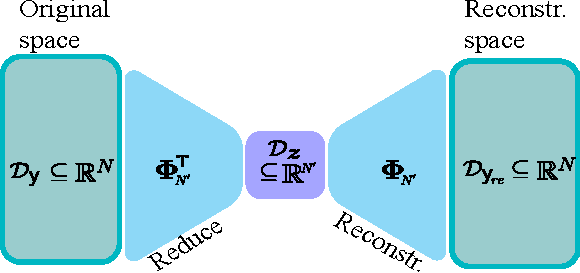
\includegraphics[width=90mm]{main_images/figure-PCA.pdf}
 \caption{ROM}
 \label{fig: ROM}
\end{figure}

Two commonly used approaches for high-dimensional spatial data are ROM and CNN. ROM techniques, such as proper orthogonal decomposition, reduce dimensionality by projecting outputs onto dominant eigenspaces identified via singular value decomposition, as illustrated in \Cref{fig: ROM}. The output is thus compressed into a latent space, with the number of retained modes determined by reconstruction accuracy. Spatial correlations are implicitly captured by the corresponding eigenvectors $\Phi$. Similarly, CNN learn nonlinear spatial representations through hierarchical filters, as shown in \Cref{fig: CNN}. Compared with ROM, the latent space in CNN is not necessarily of reduced dimensionality. Spatial structures are captured through convolution kernels and learned weights, and reconstruction is achieved via upsampling operations. While ROM and CNN handle spatial data using different algorithms, both operate within latent space. However, ROM requires an explicit DR technique, such as PCA, which could become challenging when output data is in tensor form, irregular, or of unequal length. Therefore, this study adopts a CNN-based method to capture complex nonlinear spatial patterns due to its greater flexibility. At the same time, a ROM approach is implemented as a baseline for comparison.
\begin{figure}
\centering
 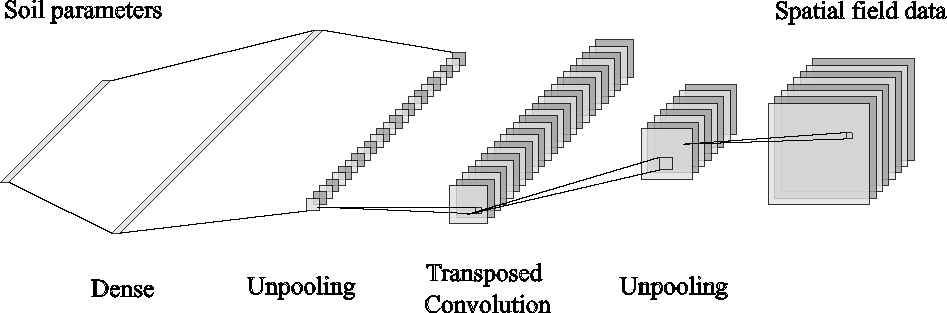
\includegraphics[width=90mm]{main_images/figure-CNN.pdf}
 \caption{CNN architecture}
 \label{fig: CNN}
\end{figure}




\subsection{Modelling temporal correlations via memory mechanisms}\noindent
LSTM networks are a specialised type of recurrent neural network designed to mitigate the vanishing gradient problem and to capture long-term dependencies in sequential data. As illustrated in \Cref{fig: LSTM}, the architecture comprises a memory cell regulated by three gates, input, forget, and output, that govern the flow of information. This design enables LSTM to retain and utilise relevant features across extended time horizons, making them particularly effective in sequence modelling tasks such as time series forecasting, stress history representation, and long-term monitoring \parencite{yu2015,benabou2021,qiu2025}.

In typical geotechnical modelling, input parameters such as soil properties are static, while outputs evolve over time. This discrepancy limits the applicability of standard LSTM networks, which require sequential inputs. To overcome this, a decoder-only architecture is developed to generate temporal responses conditioned on static inputs. This enables efficient emulation of time-dependent behaviour without relying on input sequences. Further details follow.
\begin{figure}
\centering
 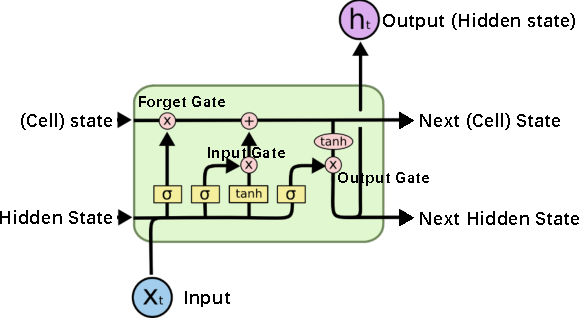
\includegraphics[width=90mm]{main_images/figure-LSTM.pdf}
 \caption{LSTM architecture}
 \label{fig: LSTM}
\end{figure}





\subsection{Simplified strategy to multi-field, multi-stage outputs}\noindent
As illustrated in \Cref{fig: decoder_only}, the static inputs are first transformed via fully connected layers to enrich and align features, then replicated across time steps before being passed to LSTM layers that capture temporal dependencies and produce latent sequences. These latent representations form an information bottleneck that bridges temporal decoding and spatial reconstruction. Spatial decoding is performed by specialised 1D or 2D convolution neural networks according to the output field type, with a TimeDistributed wrapper ensuring consistent decoding across time. When there is scalar output showing no spatial feature, only time-dependent layer is used. This modular separation of temporal and spatial components allows efficient and interpretable learning of evolving field patterns. Unlike typical sequence-to-sequence or encoder-decoder architectures (e.g., image sequences or climate fields), which encode time-varying inputs, the simplified design avoids unnecessary complexity by directly conditioning sequence generation on static inputs. Joint training of multiple output fields through a unified loss promotes balanced and coherent predictions. 

\begin{figure}
\centering
 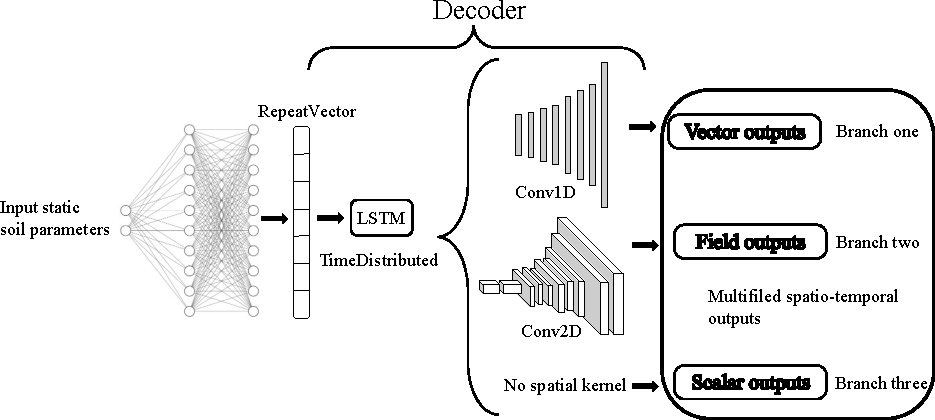
\includegraphics[width=140mm]{main_images/figure_NN.pdf}
 \caption{Decoder-only NN architecture}
 \label{fig: decoder_only}
\end{figure}


It is noted here different with ROM-surrogate frameworks \parencite{yang2024}, the proposed method avoids the two-step procedure of dimensionality reduction followed by surrogate modelling. This arises from the need to handle field outputs with non-uniform sequence lengths, as conventional reduction methods (e.g., principal component analysis, singular value decomposition) necessitate flattening the outputs into one-dimensional vectors, thereby disrupting their internal structure \parencite{sirovich1987,holmes2012}. Even advanced tensor-reduction techniques face compatibility issues with existing surrogate models, as the reduced formats are dimensionally inconsistent and ultimately still require flattening \parencite{kolda2009}. The proposed approach aims to offer greater practicality and ease of implementation for engineers.


In standard encoder-decoder formulations, the encoder is used to compress (or project) high-dimensional inputs and extract latent features, while the decoder reconstructs the high-dimensional outputs from latent representations. Such designs are well suited to problems with complex or structured inputs. However, many geotechnical engineering applications involve low-dimensional static inputs, such as soil parameters, for which an explicit encoding stage for input compression may be not essential. The proposed model therefore adopts a simplified (encoder-free) formulation in which static inputs are directly mapped into a latent representation, temporal dependencies are captured, and spatio-temporal responses are generated through the decoding components. It reflects that the primary modelling effort lies in decoding the latent representation into complex spatio-temporal outputs, rather than in performing deep feature extraction on the inputs.

\subsection{Testing the surrogate through a sequential inversion process}\label{sec: SBI}\noindent
The use of probabilistic back-analysis based on observations in geotechnical projects has been widely reported \parencite{hsein2013, lo2019, jin2021}. Among the different inverse approaches, such as maximum likelihood, maximum a posterior estimation and Monte Carlo simulation, Bayesian updating is regarded as particularly attractive for reducing uncertainties in soil parameters. Bayesian inference provides a rigorous probabilistic framework in which prior knowledge is combined with a limited number of observations. In this setting, soil parameters are treated as random vectors, with realisations denoted by $x$. The corresponding output responses are collected in a vector $y \in \mathbb{R}^{N}$, where $N$ is the length of the output. By applying the \textit{sum rule} and \textit{product rule} of probabilistic theory, the posterior distribution of the parameters $x$ can be expressed as:
\begin{equation}
\pi(x|y) = \frac{{\mathcal{L}(x|y) \cdot \pi(x)}}{{\pi(y)}} \label{equation Bayes},
\end{equation}
This expression, commonly known as \textit{Bayes' theorem}, defines the posterior distribution $\pi(x|y)$ in terms of the prior $\pi(x)$, the likelihood $\mathcal{L}(x|y)\stackrel{\mathrm{def}}{=}\pi(y|x)$
and the normalising constant, or evidence $\pi(y)$.

\Cref{equation Bayes} is rarely used, as computing the evidence $\pi(y)$ is typically intractable due to model complexity or high computational cost. Thus, methods which can approximate the posterior distribution are used. One common approach is to directly sample the posterior distribution using a Markov Chain Monte Carlo (MCMC) sampling algorithm \parencite{andrieu2003}. To avoid the computational burden of sampling using the forward model, MCMC simulations use a surrogate to construct a Markov chain ($x^{(1)}, x^{(2)}, \cdots )$ over the prior support $\mathcal{D}_{\boldsymbol{x}}$. In this study, the \textit{affine-invariant ensemble sampler} algorithm was used to construct the Markov chains with a burn-in period of 70\%. To speed up the inversion process and also at the same time verify the performance of the constructed surrogate, the surrogate model $\tilde{\mathcal{M}}(x)$ is embedded in the likelihood function. Assume that the \textit{uncertainty noise} term $\varepsilon_{r}$ follows a zero mean multivariate Gaussian distribution, i.e., $\varepsilon_{r} \sim \mathcal{N}(0,\Sigma_{\varepsilon_{r}})$. Given $m$ sets of observations and following the construction of an appropriate surrogate $\tilde{\mathcal{M}}(x)$, the likelihood can be explicitly expressed as:
\begin{equation} 
 \label{eq: modified_Likelihood function}
\begin{aligned}
 \mathcal{L}(x|\mathcal{Y}) =& \prod_{i=1}^{m} N(y^{(i)}|\tilde{\mathcal{M}}(x),\Sigma_{\varepsilon_{r}}) \\
 =& \prod_{i=1}^{m}\frac{1}{\sqrt{(2 \pi)^{N}{\rm{det}} 
 (\Sigma_{\varepsilon_{r}})}}\exp\left(-\frac{1}{2}\left[y^{(i)} - \tilde{\mathcal{M}}(x)\right]^{\mathsf{T}} \Sigma_{\varepsilon_{r}}^{-1}\left[y^{(i)} - \tilde{\mathcal{M}}(x)\right]\right) ,
\end{aligned}
\end{equation} 
\noindent The noise covariance matrix, $\Sigma_{\varepsilon_{r}}$, is mostly unknown and may be treated as additional unknowns that can be inferred jointly with the forward soil parameters. To characterise the noise, a diagonal covariance matrix of the form $\Sigma_{\varepsilon_{r}} = \sigma^2 \times \mathbf{I}$ with an unknown residual variance $\sigma^2$ is adopted, where $\mathbb{I}$ denotes an identity matrix. Although more complex noise representations exist and can be considered, this study adopts the simplest form for clarity and demonstration purposes \cite{hsein2013,lo2019}. For further details on sequential Bayesian calibration and uncertainty quantification, refer to \cite{yang2026}. 


In practice, geotechnical construction is typically carried out in stages, and it is therefore natural to employ a recursive updating strategy that reflects the sequential nature of the works. Within this framework, a sequential Bayesian calibration scheme can be applied, whereby soil parameters are progressively updated as additional observational data become available. This process allows the evolving parameter estimates to be incorporated into subsequent analyses, leading to predictions of key outputs, such as wall deflections or ground movements, with progressively reduced uncertainty at each stage of loading or excavation, as illustrated in \Cref{fig: SBI}. The updating can be repeated throughout the construction process, thereby providing a consistent mechanism to refine soil parameters and improve predictive confidence until project completion. It should be noted, however, that the initial generation of the training database relies on these FE simulations, and this upfront computational effort cannot be avoided; the surrogate and subsequent UQ analyses are inherently based on the results of high-fidelity FEM.

\begin{figure}
\centering
 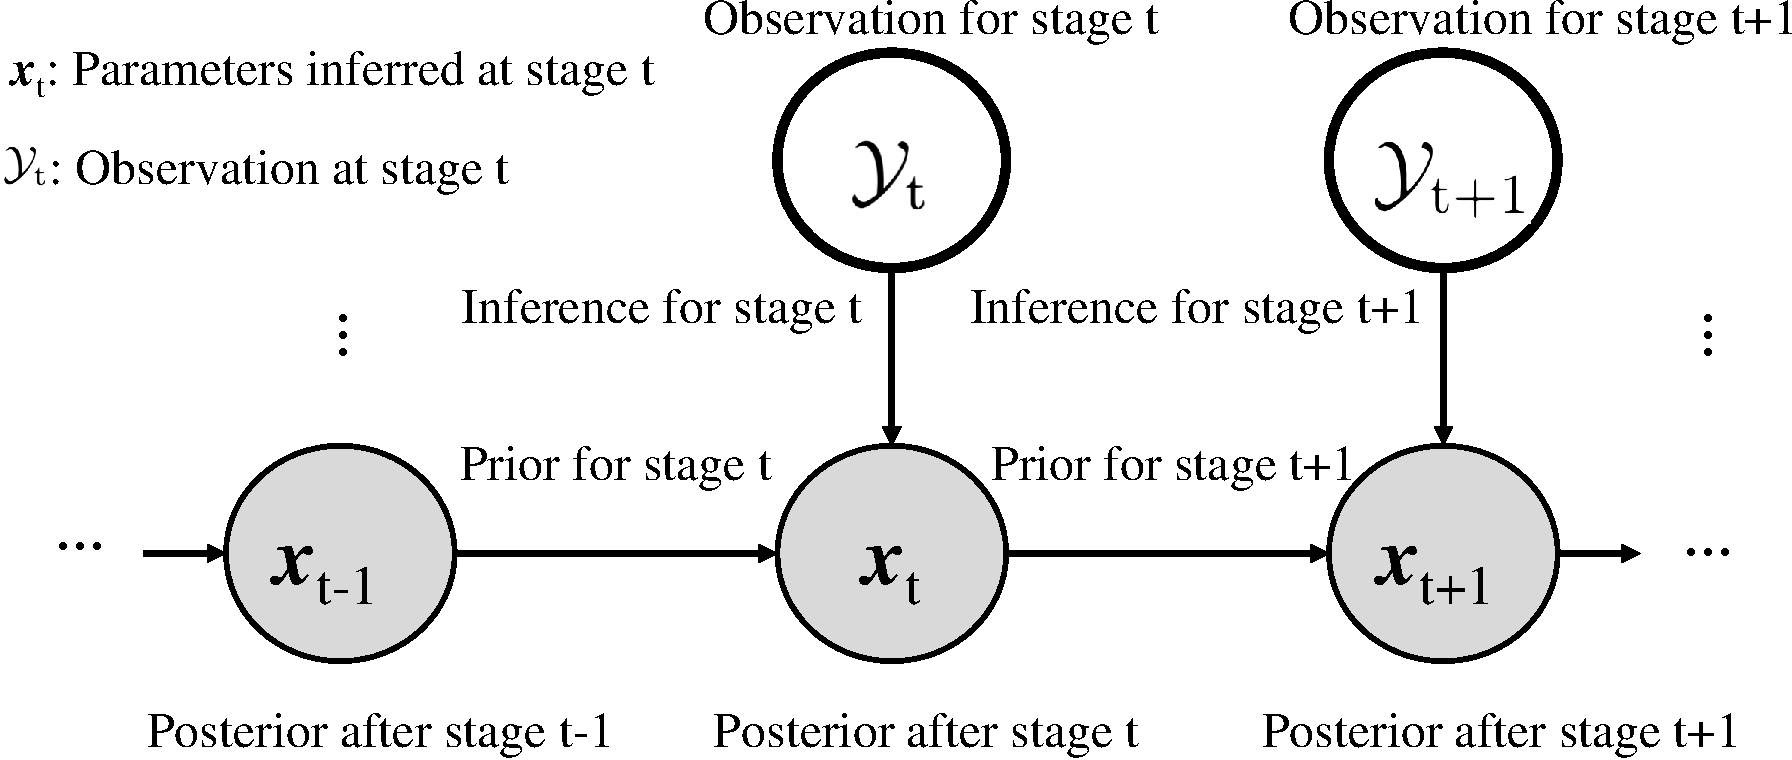
\includegraphics[width=90mm]{main_images/figure-SBI.pdf}
 \caption{Sequential Bayesian inference}
 \label{fig: SBI}
\end{figure}




















%\input{03_ComputationalDetails.tex}
\section{Benchmark problem 1: offshore strip footing loading}\label{sec:example1}\noindent
\subsection{FE model setup}\noindent
To evaluate the proposed metamodel, a strip footing loading problem on silty sand was considered, featuring low-dimensional static inputs and high-dimensional, multi-stage, multi-field outputs. Numerical simulations were performed using the commercial software ABAQUS \parencite{abaqus2022}. The model geometry and mesh configuration are shown in \Cref{fig: Mesh}, where the strip footing is represented by an equivalent surface loading \parencite{houlsby1999,xiao2018,haghighi2019}. The footing width is $D = 1.9$ m, and the soil-footing interface is assumed rough without separation, consistent with the undrained condition \parencite{yang2021,huang2021,yang2022,zhou2023,yang2024,peng2025,wang2025} . The soil layer is idealised as homogeneous, governed by a Mohr Coulomb failure criterion under total stress analysis. Loading is applied via prescribed loading, divided into nine increments of 7 kPa each, representing multi-stage loading. To minimise boundary effects, domain extents are set as $B_V=3D$ vertically and $B_H=4.5D$ horizontally. A mesh convergence study indicated that a minimum element size of $0.05D$ was sufficient for accuracy. Plane strain conditions were assumed, and the soil domain was discretised using 4-node bilinear quadrilateral elements. Boundary conditions were applied by fixing the bottom and lateral edges, while symmetry was enforced along the model centre-line using roller constraints. A geostatic equilibrium step was first performed to establish the initial in-situ stress field under gravity. The displacement field was subsequently reset to zero prior to applying the strip footing load, ensuring that the computed response corresponds solely to the applied loading.
\setcounter{figure}{5} 

To construct the metamodel, two geotechnical parameters were considered as input variables: the elastic modulus stiffness ratio, $E/s_u \sim \mathcal{U}(40,\ 2000)$, and the undrained shear strength, $s_u \sim \mathcal{U}(8\ \mathrm{kPa},\ 50\ \mathrm{kPa})$. The remaining non-linear parameters were kept constant, with the friction angle and dilation angle fixed at 28$^\circ$ and 2$^\circ$, respectively. Two output regions were extracted from the numerical results at each loading stage: (i) the ground surface zone adjacent to the footing and (ii) the subsoil zone directly beneath the footing. The former yields a vector-based output comprising 21 nodes along the surface, while the latter provides a field-based output defined over a $21 \times 17$ grid in the vertical cross-section. Each simulation consists of 9 loading increments, resulting in two output tensors:
$\tilde{\mathcal{M}}: x \in \mathbb{R}^{1 \times 2}  \rightarrow 
\mathcal{G}^{(1)} \in \mathbb{R}^{9*21}$ for surface vectors, and
$\tilde{\mathcal{M}}: x \in \mathbb{R}^{1 \times 2}  \rightarrow 
\mathcal{G}^{(2)} \in \mathbb{R}^{9*21*17} $ for subsoil fields,
where $\mathbb{R}^{1 \times 2}$ represents the input space defined by $E/s_u$ and $s_u$. $\mathcal{G}$ denotes the type of different fields of output quantities. This benchmark problem is designed to demonstrate the metamodel’s ability to capture spatially and temporally evolving geotechnical responses. 

While the current model setup considers only two input parameters ($E/s_u$ and $s_u$) and assumes a homogeneous soil layer, this simplification serves as a proof-of-concept to validate the proposed method on a simplified offshore strip footing scenario. The framework can easily extend and readily accommodate additional geotechnical input parameters, more complex constitutive models, non-linear relationships, as well as spatial variability and stratified or heterogeneous ground conditions in future applications.
\begin{figure}
\centering
 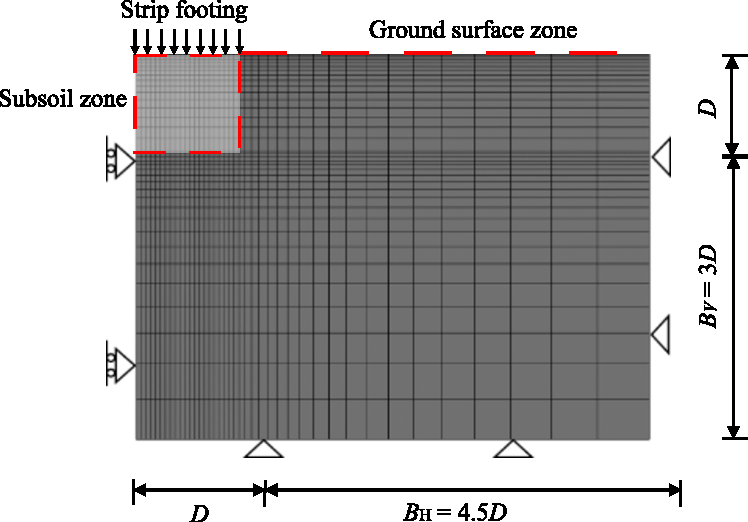
\includegraphics[width=90mm]{main_images/figure-stripfooting.pdf}
 \caption{FE model}
 \label{fig: Mesh}
\end{figure}



\subsection{Metamodel details}\noindent
The metamodel architecture is shown in \Cref{tab:nn_architecture1}. It begins with a fully connected layer comprising 50 hidden units, which maps the static input parameters into a latent feature space. The resulting latent representation is repeated across the nine loading stages and fed into an LSTM module to capture temporal dependencies. The LSTM output is then decoded into two separate branches corresponding to the two output types. Latin Hypercube sampling was used to generate 350 samples from the defined parameter space $\mathcal{D}_{\boldsymbol{x}}$. For all simulations, the dataset is partitioned using a fixed random seed. For the learning-curve analysis, subsets corresponding to 16\%, 24\%, 32\%, 40\% and 80\% of the full dataset are used for training, while the remaining 20\% samples form a fixed test set and are not used during training. The input parameters and model responses are then normalised to $[0,1]$ globally using a min-max transformation, with the scaling factors estimated from the training pool and applied unchanged to the test set. For each response quantity, the spatio-temporal tensors are flattened to arrays of size $(n_{\text{sample}}, N_{\text{dof}})$ prior to scaling and subsequently reshaped to their original dimensions.



The first branch reconstructs the ground surface settlement $\mathcal{G}^{(1)}$ using a sequence of time-distributed transposed 1D convolution layers. The latent sequence is first passed through a dense layer of 320 units and reshaped into a temporal sequence, followed by convolution layers with kernel size 3, stride 2, and ReLU activation. The second branch reconstructs the subsoil displacement field $\mathcal{G}^{(2)}$ using time-distributed transposed 2D convolution layers. The latent vector is first expanded through a dense layer into a spatial tensor, then reshaped and processed by convolution layers with 64, 32, 16, and 1 filters, all with kernel size 3, stride 1, and 'same' padding. ReLU activation is used for all layers except the final one, which uses linear activation to preserve continuous field values. Both branches are trained jointly using a unified loss function and Adam optimiser on \texttt{Tensorflow} API, allowing consistent learning across vector and field outputs. The hyperparameters, such as the number of hidden units, were empirically chosen based on the complexity of the task and the dimensionality of the output sequences. This choice balances predictive accuracy and hyper-parameter tuning complexities. Although further optimisation could improve performance, this configuration suffices to demonstrate the method's feasibility. It is noted that no explicit physics constraints, such as those in Physics-Informed Neural Networks, were used; however, the outputs were checked for physical plausibility. Convergence challenges, which may arise in geotechnical problems with large displacements or non-linear behaviour, could be addressed by adjusting step sizes and refining the mesh in critical regions.
\begin{table}[t]
\centering
\caption{Neural network architecture and parameter counts for offshore strip footing problem}
\label{tab:nn_architecture1}
\small
\setlength{\tabcolsep}{5pt}
\begin{tabular}{lll r}
\toprule
Layer & Type & Output shape & Params \\
\midrule
Input & InputLayer & (None, 2) & 0 \\
Dense & Dense(50) & (None, 50) & 150 \\
Repeat & RepeatVector(9) & (None, 9, 50) & 0 \\
LSTM & LSTM(50), return\_seq & (None, 9, 50) & 20{,}200 \\
\midrule
\multicolumn{4}{c}{\textbf{Branch A: displacement vector output}} \\
\midrule
TD-Dense & TimeDistributed(Dense(320)) & (None, 9, 320) & 16{,}320 \\
TD-Reshape & TimeDistributed(Reshape) & (None, 9, 10, 32) & 0 \\
TD-Conv1DT & TimeDistributed(Conv1DTranspose(1)) & (None, 9, 21, 1) & 97 \\
Output-A & Lambda (squeeze) & (None, 9, 21) & 0 \\
\midrule
\multicolumn{4}{c}{\textbf{Branch B: displacement field output}} \\
\midrule
TD-Dense & TimeDistributed(Dense(1344)) & (None, 9, 1344) & 68{,}544 \\
TD-Reshape & TimeDistributed(Reshape) & (None, 9, 16, 21, 4) & 0 \\
TD-Conv2DT-1 & TimeDistributed(Conv2DTranspose(64)) & (None, 9, 16, 21, 64) & 2{,}368 \\
TD-Conv2DT-2 & TimeDistributed(Conv2DTranspose(32)) & (None, 9, 16, 21, 32) & 18{,}464 \\
TD-Conv2DT-3 & TimeDistributed(Conv2DTranspose(16)) & (None, 9, 16, 21, 16) & 4{,}624 \\
TD-Conv2DT-4 & TimeDistributed(Conv2DTranspose(1)) & (None, 9, 16, 21, 1) & 145 \\
Output-B & Lambda (squeeze) & (None, 9, 16, 21) & 0 \\
\midrule
\textbf{Total} &  &  & \textbf{130{,}912} \\
\bottomrule
\end{tabular}
\end{table}

\subsection{Baselines}\noindent
To evaluate the predictive capability of the proposed surrogate model, comparisons are conducted against several established baseline approaches in order to place its performance in context. All models are trained and assessed using the same dataset partitioning and evaluation metrics to ensure consistency. As a representative reduced-order modelling (ROM) strategy, a PCA-PCE framework is adopted. In this approach, principal component analysis (PCA) is employed as a matrix-based dimensionality reduction technique to extract dominant modes from the high-dimensional output field; the spatial outputs are therefore flattened prior to decomposition and reshaped back to their original configuration after reconstruction. Polynomial chaos expansion (PCE) is subsequently used to establish the mapping between input parameters and the reduced coefficients, following the implementation described in \cite{yang2026}. In addition to this baseline, component-wise model configurations of the proposed architecture are constructed to examine the contributions of individual components. Specifically, the LSTM layers are removed to assess the role of temporal feature extraction in capturing time-dependent behaviour, while a separate variant without convolution layers is developed to evaluate the influence of CNN-based spatial feature learning on representing complex spatial patterns and local interactions within the predicted field. These controlled comparisons enable the respective contributions of reduced-order modelling, temporal learning, and spatial feature extraction to be examined in a consistent framework.


\subsection{Metamodel performance}\noindent
The predictive performance of the metamodel is quantified by comparison with reference simulations using the \textit{Global Normalised Absolute Error} (GNAE, a normalised $L_1$ type error), \textit{Mean Absolute Error} (MAE) and \textit{Relative $L_2$ Error} ($L_2$ type error) \parencite{chai2014,mendo2009,zhu2019}, defined as follows:
\begin{equation}
 \text{GNAE} = \frac{1}{K'} \sum_{k=1}^{K'} \frac{ \left| \mathcal{M}(x_k) - \tilde{\mathcal{M}}(x_k) \right| } {\max(\mathcal{M}(x_k)) - \min(\mathcal{M}(x_k))} \times 100 , 
\end{equation}
\begin{equation}
\text{MAE}
=
\frac{1}{K'}
\sum_{k=1}^{K'}
\left|
\mathcal{M}(x_k) - \tilde{\mathcal{M}}(x_k)
\right|, 
\end{equation}
\begin{equation}
\text{Relative } L_2
=
\frac{
\sqrt{
\sum_{k=1}^{K'}
\left(
\mathcal{M}(x_k)
-
\tilde{\mathcal{M}}(x_k)
\right)^2
}
}
{
\sqrt{
\sum_{k=1}^{K'}
\left(
\mathcal{M}(x_k)
\right)^2
}
}
, 
\end{equation}
where $K'$ denotes the number of FE simulations in the test set, $\mathcal{M}(x)$ represents the FE predictions, and $\tilde{\mathcal{M}}(x)$ denotes the corresponding metamodel outputs. The GNAE provides a scale-independent percentage measure by normalising the absolute error with respect to the global range of the reference solution. This normalisation enhances robustness when the solution magnitude varies significantly across the domain and reduces the influence of disproportionately large local deviations. The MAE quantifies the average magnitude of pointwise prediction errors, offering a direct and physically interpretable assessment of absolute deviation. It reflects the typical local discrepancy between the predicted and reference values without overemphasising extreme errors. The Relative $L_2$ error evaluates the global error in an energy-norm sense by considering the squared differences between prediction and reference.

The evolution of the loss over training epochs is illustrated in \Cref{fig: loss}, where a logarithmic scale is employed to emphasise the rapid reduction in the early stages of training. As expected, the total loss decreases progressively, spanning approximately three orders of magnitude over the entire training period. The loss associated with $\mathcal{G}^{(1)}$ stabilises relatively quickly, likely due to the lower spatial complexity and smoother nature of its output, which is a vector. In contrast, the loss corresponding to $\mathcal{G}^{(2)}$ exhibits evident fluctuations and a slower convergence rate, attributable to the higher spatial complexity of the predicted field. From a physical standpoint, this behaviour is consistent with the role of $\mathcal{G}^{(2)}$ in capturing complex and spatially detailed variations within the subsoil displacement field. Despite these challenges, the overall trend, along with the eventual plateauing of the loss, indicates that the model has reached convergence.

The test performance of the different surrogate models under varying training sample sizes is summarised in \Cref{tab:test_error1,tab:test_error2,tab:test_error3}. For both the vector-valued response $\mathcal{G}^{(1)}$ and the field-type response $\mathcal{G}^{(2)}$, a general reduction in all three error measures (GNAE, MAE and $L_2$) is observed as the number of training samples increases, indicating that all models benefit from additional high-fidelity data. In which, the PCA-PCE model performs reasonably well at smaller sample sizes but its accuracy improves only modestly as further data are added, suggesting that its capacity to capture the strong non-linearity and spatio-temporal coupling in the present problem is limited. The comparison among the three neural-network baselines further clarifies the role of the different components in the proposed architecture: the CNN+MLP configuration without LSTM systematically underperforms the recurrent variants, highlighting that neglecting temporal dynamics leads to an inferior representation of sequence-dependent responses, whereas the “LSTM Only” configuration improves the treatment of temporal correlations but, owing to the absence of an explicit convolution layer, lacks the ability to efficiently exploit spatial structure and therefore yields an intermediate level of accuracy between CNN+MLP and the full proposed model. Overall, these observations indicate that the proposed architecture is necessary to exploit both spatial and temporal dependencies effectively. Three complementary error measures, GNAE, MAE and the $L_2$, are employed to mitigate the risk of drawing misleading conclusions from a single metric; although their absolute magnitudes differ, they provide consistent rankings of the competing surrogates over all sample sizes and for both output types, thereby offering a robust assessment of the superiority and reliability of the proposed model. \Cref{fig: fitting} shows regression plots comparing the metamodel predictions of $\mathcal{G}^{(1)}$ and $\mathcal{G}^{(2)}$ with the corresponding reference values for both training and test datasets, with the diagonal line indicating perfect agreement. In all cases, the points lie in a narrow band around the identity line, and no systematic bias, trend reversal or noticeable outliers can be observed between training and test sets, suggesting that over-fitting is negligible.  

\begin{figure}
\centering
 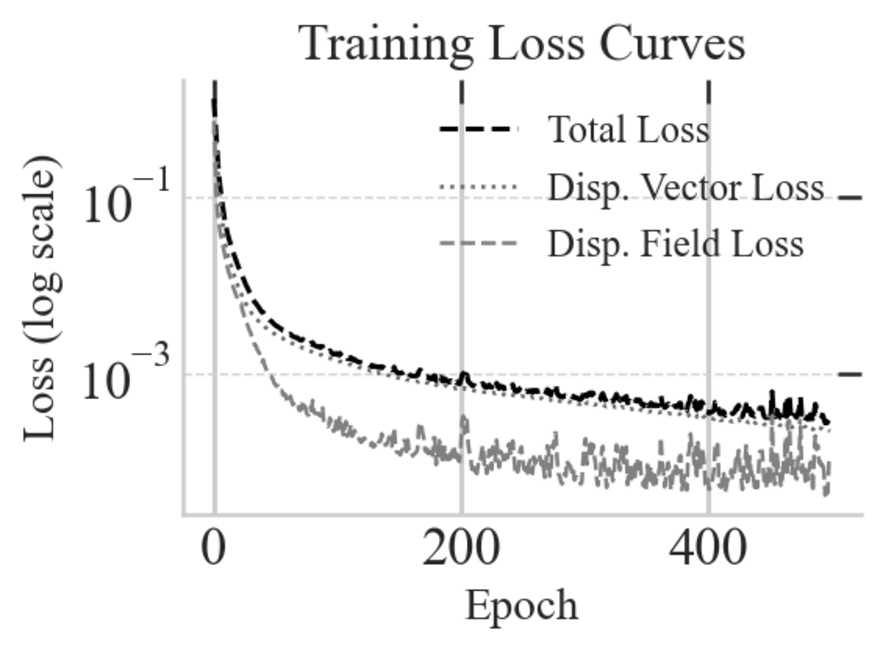
\includegraphics[width=90mm]{main_images/figure-loss.pdf}
 \caption{Training loss curves for total and output-specific losses}
 \label{fig: loss}
\end{figure}




\begin{table}[htbp]
\centering
\caption{GNAE of different surrogate models under varying training sample sizes}
\label{tab:test_error1}
\sisetup{
    table-format=3.2,
    detect-weight=true,
    detect-inline-weight=math
}
\begin{tabular}{c l S S S S}
\toprule
\multirow{2}{*}{Samples} & \multirow{2}{*}{Case} & 
\multicolumn{4}{c}{Test Error (\%)} \\
\cmidrule(lr){3-6}
 &  & {Proposed} & {PCA--PCE} & {CNN+MLP (No LSTM)} & {LSTM Only} \\
\midrule
56  & $\mathcal{G}^{(1)}$ & 4.05 & 4.21 & 9.80 & 5.02 \\
84  & $\mathcal{G}^{(1)}$ & 2.30 & 3.38 & 10.78 & 4.24 \\
112 & $\mathcal{G}^{(1)}$ & 2.01 & 3.10 & 10.70 & 2.51 \\
140 & $\mathcal{G}^{(1)}$ & 1.56 & 3.00 & 9.86 & 2.87 \\
280 & $\mathcal{G}^{(1)}$ & 1.27 & 3.24 & 7.36 & 3.03 \\
\midrule
56  & $\mathcal{G}^{(2)}$ & 5.50 & 7.16 & 8.57 & 5.65 \\
84  & $\mathcal{G}^{(2)}$ & 6.17 & 4.57 & 7.32 & 3.74 \\
112 & $\mathcal{G}^{(2)}$ & 4.53 & 4.26 & 6.54 & 3.27 \\
140 & $\mathcal{G}^{(2)}$ & 6.55 & 4.15 & 6.14 & 2.81 \\
280 & $\mathcal{G}^{(2)}$ & 0.82 & 4.35 & 6.12 & 2.93 \\
\bottomrule
\end{tabular}
\end{table}


\begin{table}[htbp]
\centering
\caption{MAE of different surrogate models under varying training sample sizes}
\label{tab:test_error2}
\sisetup{
    table-number-alignment = center,
    table-format = 1.2
}
\begin{tabular}{c c S S S S}
\toprule
\multirow{2}{*}{Samples} & \multirow{2}{*}{Case} &
\multicolumn{4}{c}{Test Error} \\
\cmidrule(lr){3-6}
 & & {Proposed} & {PCA--PCE} & {CNN+MLP (No LSTM)} & {LSTM Only} \\
\midrule
56  & $\mathcal{G}^{(1)}$ & 0.07 & 0.07 & 0.17 & 0.09 \\
84  & $\mathcal{G}^{(1)}$ & 0.04 & 0.06 & 0.19 & 0.07 \\
112 & $\mathcal{G}^{(1)}$ & 0.03 & 0.05 & 0.18 & 0.04 \\
140 & $\mathcal{G}^{(1)}$ & 0.03 & 0.05 & 0.17 & 0.05 \\
280 & $\mathcal{G}^{(1)}$ & 0.02 & 0.05 & 0.13 & 0.04 \\
\midrule
56  & $\mathcal{G}^{(2)}$ & 0.39 & 0.51 & 0.61 & 0.40 \\
84  & $\mathcal{G}^{(2)}$ & 0.44 & 0.32 & 0.52 & 0.27 \\
112 & $\mathcal{G}^{(2)}$ & 0.32 & 0.30 & 0.46 & 0.23 \\
140 & $\mathcal{G}^{(2)}$ & 0.47 & 0.29 & 0.43 & 0.20 \\
280 & $\mathcal{G}^{(2)}$ & 0.06 & 0.30 & 0.23 & 0.18 \\
\bottomrule
\end{tabular}
\end{table}


\begin{table}[htbp]
\centering
\caption{$L_2$ of different surrogate models under varying training sample sizes}
\label{tab:test_error3}
\sisetup{
    table-number-alignment = center,
    table-format = 1.2
}
\begin{tabular}{c c S S S S}
\toprule
\multirow{2}{*}{Samples} & \multirow{2}{*}{Case} &
\multicolumn{4}{c}{Test Error} \\
\cmidrule(lr){3-6}
 & & {Proposed} & {PCA--PCE} & {CNN+MLP (No LSTM)} & {LSTM Only} \\
\midrule
56  & $\mathcal{G}^{(1)}$ & 0.09 & 0.05 & 0.12 & 0.10 \\
84  & $\mathcal{G}^{(1)}$ & 0.03 & 0.04 & 0.11 & 0.04 \\
112 & $\mathcal{G}^{(1)}$ & 0.03 & 0.03 & 0.10 & 0.03 \\
140 & $\mathcal{G}^{(1)}$ & 0.02 & 0.04 & 0.10 & 0.03 \\
280 & $\mathcal{G}^{(1)}$ & 0.01 & 0.04 & 0.08 & 0.03 \\
\midrule
56  & $\mathcal{G}^{(2)}$ & 0.10 & 0.07 & 0.11 & 0.11 \\
84  & $\mathcal{G}^{(2)}$ & 0.05 & 0.04 & 0.06 & 0.04 \\
112 & $\mathcal{G}^{(2)}$ & 0.04 & 0.04 & 0.06 & 0.03 \\
140 & $\mathcal{G}^{(2)}$ & 0.05 & 0.04 & 0.06 & 0.03 \\
280 & $\mathcal{G}^{(2)}$ & 0.01 & 0.04 & 0.07 & 0.03 \\
\bottomrule
\end{tabular}
\end{table}


As an illustration, \Cref{fig: output} shows representative responses of both the metamodel and the forward model in the original output space. For the vector-type output $\mathcal{G}^{(1)}$, \Cref{fig: output}(a) demonstrates that the predicted profiles (red lines) align well with the reference FE results (black lines) over all loading stages, correctly reproducing both the magnitude and the shape of the settlement. For the field-type output $\mathcal{G}^{(2)}$, \Cref{fig: output}(b) shows the numerical model displacement fields, the corresponding metamodel prediction and their point-wise differences at three representative stages (1, 5 and 9). As the load increases, the true fields exhibit a progressive expansion and deepening of the deformation zone beneath and around the footing, and the metamodel closely follows this evolution. The error maps show small, spatially scattered residuals with no evident systematic bias. Overall, the agreement between the metamodel and FE solutions is satisfactory in both space and time, and the remaining discrepancies are small relative to the response magnitude and acceptable for typical geotechnical applications.

\begin{figure}[htbp]
    \centering
    \begin{subfigure}[b]{\textwidth}
        \centering
        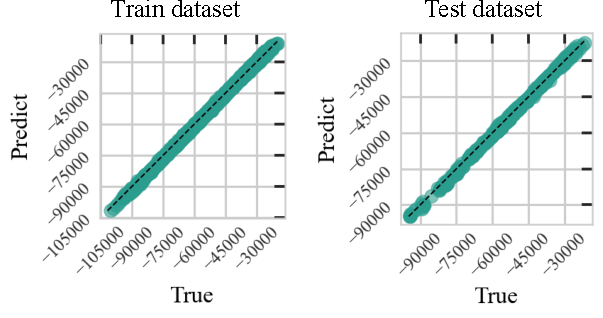
\includegraphics[width = 90mm]{main_images/figure-G1.pdf}
        \caption{$\mathcal{G}^{(1)}$}
    \end{subfigure}%
    \vfill
    \begin{subfigure}[b]{\textwidth}
        \centering
        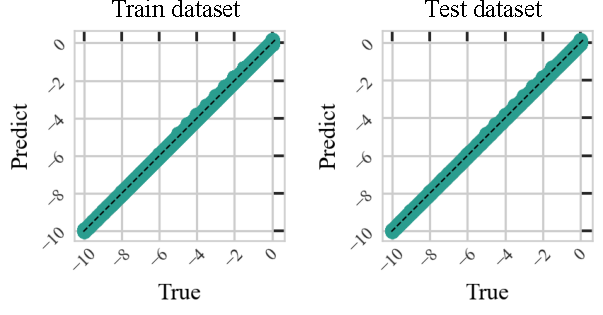
\includegraphics[width = 90mm]{main_images/figure-G2.pdf}
        \caption{$\mathcal{G}^{(2)}$}
    \end{subfigure}%
    \caption{Regression plot}
    \label{fig: fitting}
\end{figure}


To facilitate surrogate modelling and maintain reproducibility, the workflow was implemented in an end-to-end manner. Input parameters were sampled evenly using the Latin Hypercube sampling method, and for each parameter set, a FE simulation was performed to obtain the corresponding model responses. The outputs from all simulations were collected and reshaped into arrays suitable for neural network training, with vector-type responses arranged as rows and field-type outputs as matrix. The dataset was divided into training and validation subsets (80\% and 20\%, respectively) using a fixed random seed, and all inputs and outputs were scaled to the [0,1] range using min-max normalisation before training. The surrogate was trained on these preprocessed data, with a fixed seed ensuring consistent weight initialisation and mini-batch sampling. Once trained, the NN was used in a sequential calibration framework, where Markov Chain Monte Carlo sampling was performed to approximate the soil parameters' distributions; fixed seeds were applied here as well. By following this sequence, from design space sampling and FE simulation, through data reshaping, normalisation, and NN training, to surrogate-based calibration, the procedure can be reproduced under comparable computational conditions.

\begin{figure}[htbp]
    \centering
    \begin{subfigure}[b]{\textwidth}
        \centering
        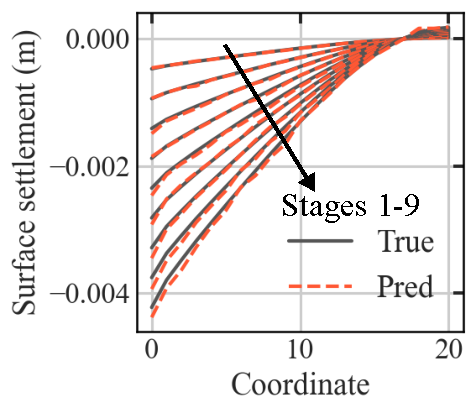
\includegraphics[width = 70mm]{main_images/figure-G1output.pdf}
        \caption{$\mathcal{G}^{(1)}$}
    \end{subfigure}%
    \vfill
    \begin{subfigure}[b]{\textwidth}
        \centering
        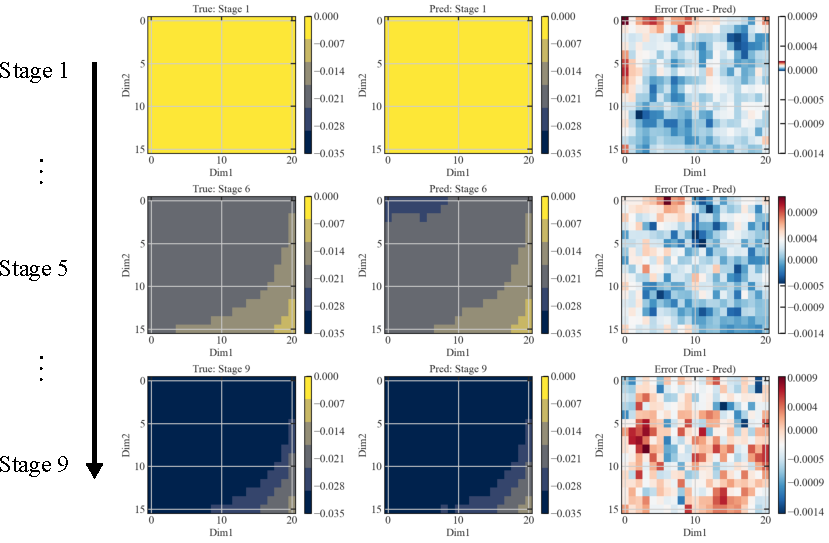
\includegraphics[width = 140mm]{main_images/figure-G2output.pdf}
        \caption{$\mathcal{G}^{(2)}$}
    \end{subfigure}%
    \caption{Metamodel performance on output space ($E$ = 12.5 MPa, $s_u$ = 9 kPa)}
    \label{fig: output}
\end{figure}
\section{Problem 2: triaxial test loading}\label{sec:example2}\noindent
\subsection{FE model setup}\noindent
The investigation focuses on a fundamental triaxial test setup with an axisymmetric soil sample confined between two parallel, rough platens. As shown in \Cref{fig: FEmodel-triaxialsetup}, the simulation models drained triaxial tests using pure displacement. The assumptions of rigid platens and soil homogeneity ensure consistent stress distribution throughout the model. The soil sample, with a radius of $R = 38$ mm and a height of $H = 140$ mm, replicates a standard triaxial sample size. A two-dimensional axisymmetric mesh with 1,330 elements was employed to simulate the soil, with each element being a 4-node axisymmetric quadrilateral (CAX4P) for pore/fluid stress. Boundary conditions were applied such that vertical and horizontal displacements at the model base were fixed ($u_y$, $u_x = 0$), and horizontal displacement was fixed along the line of symmetry ($u_x = 0$). A uniform downward displacement was incrementally applied to the top edge of the mesh, reaching a maximum of 10 mm, to simulate a strain-controlled triaxial test. This method is commonly used in Abaqus numerical simulations \parencite{helwany2007, Matthew2024}. The red dashed line representing the line of symmetry. The axisymmetric model is swept along the axis of symmetry to illustrate the 3D representation. 



The Modified Cam-Clay model, commonly used in soil mechanics, captures key clay behavior under stress \parencite{roscoe1968}. Analyses and simulations were performed using Abaqus FEA with an implicit integration scheme and the standard solver to address nonlinearity, employing the Newton-Raphson method for solution updates and convergence. Uncertain soil parameters, including $\lambda$, $\kappa$, $\mathsf{M}$, and OCR, were varied, with their ranges, units, and meanings listed in \Cref{table: input parameters}. The outputs of interest are reaction force, axial deformation, and radial deformation. To generate the dataset for metamodel training, the four governing parameters were sampled from uniform distributions and a factorial design of 340 Monte Carlo simulations was conducted using Latin hypercube sampling. A covariance of 0.85 was applied between $\kappa$ and $\lambda$ to account for their interdependence, following \parencite{Matthew2024,dawood2025}.

\begin{table}[htbp]
\centering
\caption{Priors for parameter variations}
\begin{tabular}{llll}
\hline
$x$        & $\mathcal{D}_x$                            & Unit & Physical meaning                                                                        \\ \hline
$\lambda$      & $\mathcal{U}$(0.01, 1) & --  & Logarithmic hardening modulus                                                              \\
$\kappa$ & $\mathcal{U}$(0.01,1) & --  & Logarithmic bulk modulus
                                                   \\
$\mathsf{M}$  & $\mathcal{U}$(0.5,1.4) & --  & Critical state ratio                                                                \\
$OCR$      & $\mathcal{U}$(40.0, 150.0) & --  & Overconsolidation ratio                                                   \\
\hline
\end{tabular}
\label{table: input parameters}
\end{table}

Three outputs were collected: (1) reaction forces, $\mathcal{G}^{(1)} \in \mathbb{R}^{8 \times 1}$, (2) axial deformation, $\mathcal{G}^{(2)} \in \mathbb{R}^{8 \times 71}$, and (3) radial deformations of the triaxial specimen, $\mathcal{G}^{(3)} \in \mathbb{R}^{8 \times 71}$. Each simulation consisted of 8 loading increments, resulting in a three-output tensor. Due to the inherent complexity of the Modified Cam-Clay model, the responses exhibit evident nonlinearity, as illustrated in Figure \ref{fig: priorpred}. The prior predictive distribution in panel (a) highlights the overall reaction force characteristics before metamodel construction and Bayesian calibration, while panels (b) and (c) show axial and radial deformations for a representative triaxial test. Since the last two results are vector-based, only one sample is presented here to illustrate the response, without displaying the full output uncertainty.

\begin{table}[t]
\centering
\caption{Neural network architecture and parameter counts for triaxial loading problem}
\label{tab:nn_architecture_small}
\small
\setlength{\tabcolsep}{5pt}
\begin{tabular}{lll r}
\toprule
Layer & Type & Output shape & Params \\
\midrule
Input & InputLayer & (None, 4) & 0 \\
Dense & Dense(50) & (None, 50) & 250 \\
Repeat & RepeatVector(8) & (None, 8, 50) & 0 \\
LSTM & LSTM(50), return\_seq & (None, 8, 50) & 20{,}200 \\
\midrule
\multicolumn{4}{c}{\textbf{Branch A: scalar output}} \\
\midrule
TD-Dense & TimeDistributed(Dense(50)) & (None, 8, 50) & 2{,}550 \\
Output-A & TimeDistributed(Dense(1)) & (None, 8, 1) & 51 \\
\midrule
\multicolumn{4}{c}{\textbf{Branch B: vector output (1)}} \\
\midrule
TD-Dense & TimeDistributed(Dense(71)) & (None, 8, 71) & 3{,}621 \\
TD-Reshape & TimeDistributed(Reshape) & (None, 8, 71, 1) & 0 \\
TD-Conv1D & TimeDistributed(Conv1D(1)) & (None, 8, 71, 1) & 4 \\
Output-B & Lambda (squeeze) & (None, 8, 71) & 0 \\
\midrule
\multicolumn{4}{c}{\textbf{Branch C: vector output (2)}} \\
\midrule
TD-Dense & TimeDistributed(Dense(71)) & (None, 8, 71) & 3{,}621 \\
TD-Reshape & TimeDistributed(Reshape) & (None, 8, 71, 1) & 0 \\
TD-Conv1D & TimeDistributed(Conv1D(1)) & (None, 8, 71, 1) & 4 \\
Output-C & Lambda (squeeze) & (None, 8, 71) & 0 \\
\midrule
\textbf{Total} &  &  & \textbf{32{,}851} \\
\bottomrule
\end{tabular}
\end{table}

\setcounter{figure}{9} 
\begin{figure}
\centering
 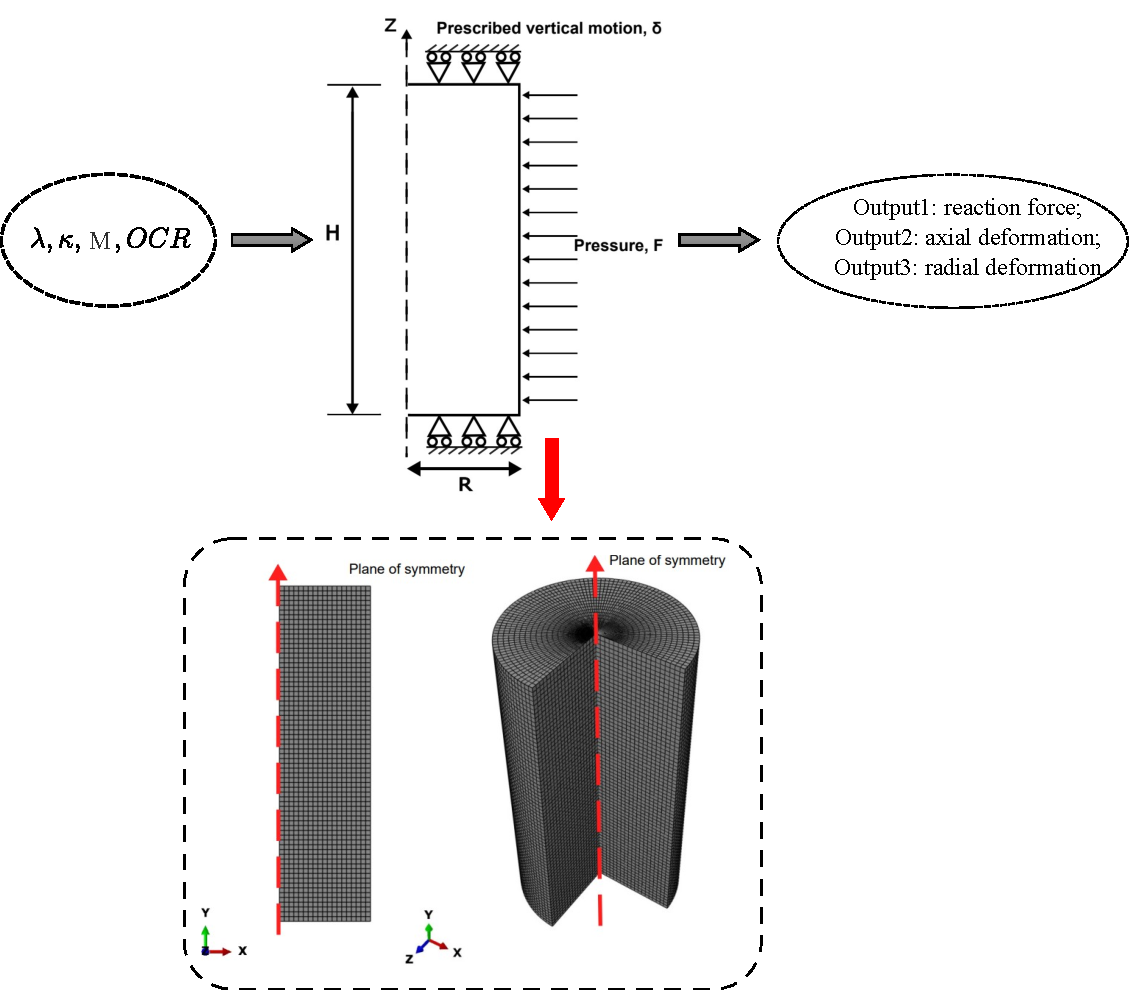
\includegraphics[width=140mm]{main_images/figure-FE-triaxial.pdf}
 \caption{Model setup}
 \label{fig: FEmodel-triaxialsetup}
\end{figure}
\begin{figure}
\centering
 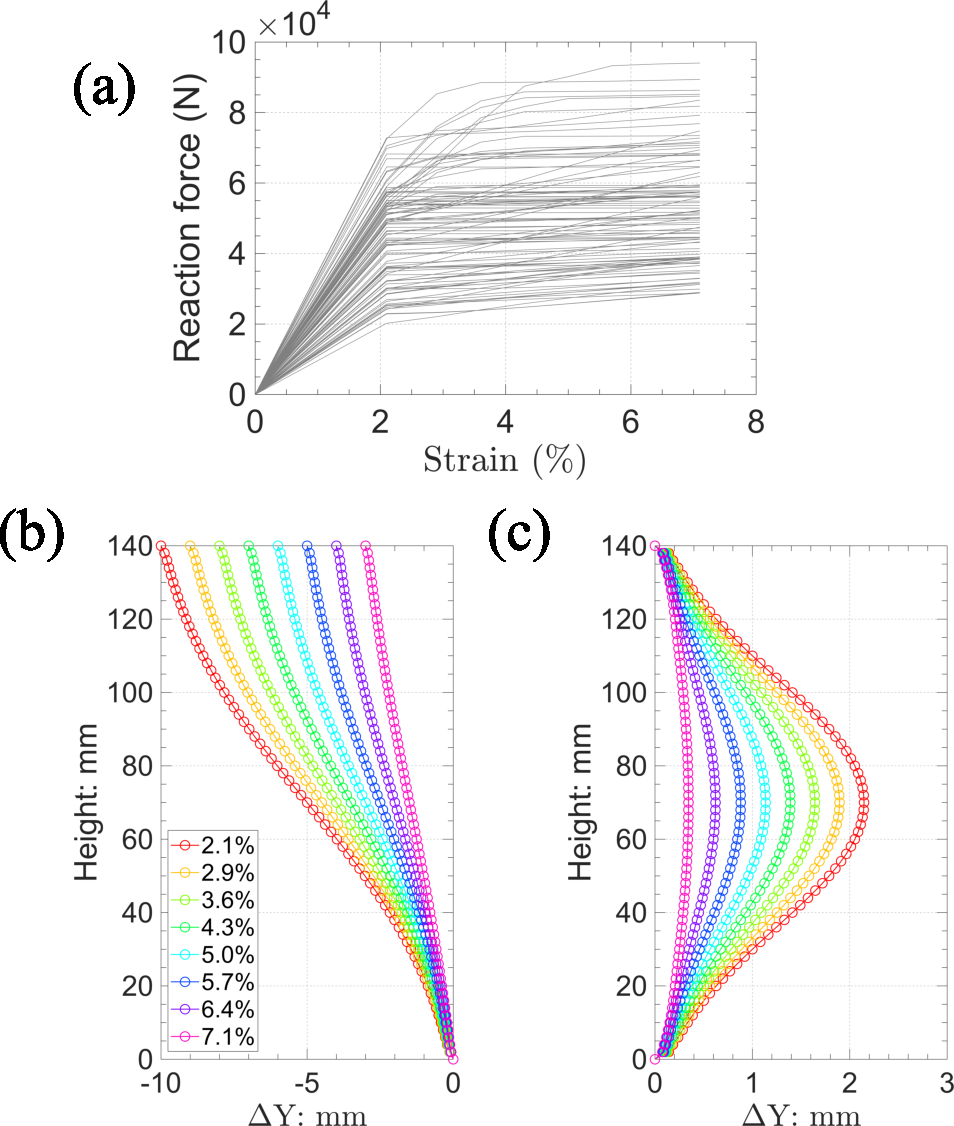
\includegraphics[width=90mm]{main_images/figure-priorpred.pdf}
 \caption{(a) Reaction force (prior predictive); (b) Axial deformation (one sample); (c) Radial deformation (one sample)}
 \label{fig: priorpred}
\end{figure}







\subsection{Metamodel construction}\noindent
80\% of the data are used for training and the remaining 20\% are reserved for testing. As shown in \Cref{tab:nn_architecture_small}, the model architecture consists of a multi-branch structure designed to predict three different outputs of the triaxial specimen. The network begins with an input layer that processes the input data into a latent feature space. This latent space is then passed through two dense layers, each with 50 hidden units, to learn meaningful representations of the input features. The resulting latent vector is then repeated across 8 loading increments, representing different loading stages, before being passed into an LSTM layer to capture temporal dependencies between these stages. The LSTM output is subsequently used as input for three distinct output branches. The first branch reconstructs the reaction forces ($\mathcal{G}^{(1)}$), with a shape of $\mathbb{R}^{8 \times 1}$, representing temporal force variations across 8 loading stages. This is achieved using time-distributed dense layers with 50 units, as there are no spatial features involved. The second branch reconstructs axial deformation ($\mathcal{G}^{(2)}$) with a shape of $\mathbb{R}^{8 \times 71}$, representing deformation across 8 stages and 71 mesh points. It uses a dense layer followed by three time-distributed transposed 1D convolution layers (kernel size 3, ReLU activation). The third branch, reconstructing radial deformation ($\mathcal{G}^{(3)}$), follows a similar approach to the second, utilising time-distributed transposed 1D convolutions to predict radial displacement over time.

\subsection{Likelihood configuration}\label{Likelihood configuration}\noindent
As shown in \Cref{eq: modified_Likelihood function}, the constructed surrogate model is embedded in the likelihood function $\mathcal{L}$ to accelerate the MCMC sampling. Since three different output types are considered, the total likelihood is taken as the product of three conditionally independent contributions,
\begin{equation}
\mathcal{L}_{\text{total}} = \mathcal{L}_{1} \times \mathcal{L}_{2} \times \mathcal{L}_{3},
\end{equation}
where $\mathcal{L}_{r}$ denotes the likelihood associated with the $r$-th output type. The observations are generated synthetically by perturbing the reference FE response with additive Gaussian noise of 3\%, so that a “ground-truth’’ data set is available and the corresponding soil parameters are known but not used either for training the surrogate model or within the MCMC procedure.

As discussed in \Cref{sec: SBI}, a Gaussian-type model is adopted for each output type. Although more elaborate or problem-specific likelihood formulations could be used, the Gaussian likelihood is chosen here for its simplicity and widespread use. For each output type $r$, the residual noise between surrogate predictions and observations is modelled as zero-mean Gaussian with diagonal covariance $\Sigma_{\varepsilon_r} = \sigma_r^{2}\mathbb{I}$. The variance $\sigma_r^{2}$ is treated as an additional unknown and inferred jointly with the soil parameters, with a weakly informative prior $\sigma_r \sim \mathcal{U}\bigl(0,\max(\mathcal{Y}_r)\bigr)$, where $\mathcal{Y}_r$ denotes the set of observations for output type $r$. This choice links the admissible noise level to the magnitude of the corresponding measurements. It should be noted that heteroscedastic noise is not modelled in this study, since only a single monitoring realisation is available and a more complex noise structure would not be identifiable in a robust manner; with richer monitoring data, heteroscedastic extensions could be introduced. All time steps and all three output types are assimilated through sequential Bayesian updating. The posterior distribution of the soil parameters and noise variances is approximated using an affine-invariant ensemble sampler with 300 chains of 300 steps each, discarding the initial 70\% of iterations as burn-in.


\subsection{Performance}\noindent
To assess the performance of the constructed metamodel, \Cref{fig: triaxialperformance} presents regression plots of predictions against reference values for both training and test datasets. The diagonal line indicates perfect agreement, and the results show good consistency. The metamodel was further evaluated within a sequential Bayesian inversion framework to test its ability to quantify uncertainty, a critical aspect in geotechnical applications. Following the procedure in \Cref{sec: SBI,Likelihood configuration}, the metamodel was embedded in the likelihood function to accelerate the inversion. One dataset sample was withheld as ground truth ($\lambda$ = 0.49, $\kappa$ = 0.06, $\mathsf{M}$ = 0.72 and $OCR$ = 130), excluded from both training and testing, and subsequently treated as synthetic observations for calibration. As shown in \Cref{fig: Cornerplot}, parameter uncertainty progressively decreases with additional observations, as expected. The predefined ground truth (black dashed lines) is approached by the posterior distributions (blue regions), with the MAP estimates (red circles) clustering closely around the true values, demonstrating the metamodel’s effectiveness in inversion. Together, these results confirm that the constructed metamodel provides both accurate predictions and reliable support for uncertainty quantification tasks.





\begin{figure}[htbp]
    \centering
    \begin{subfigure}[b]{\textwidth}
        \centering
        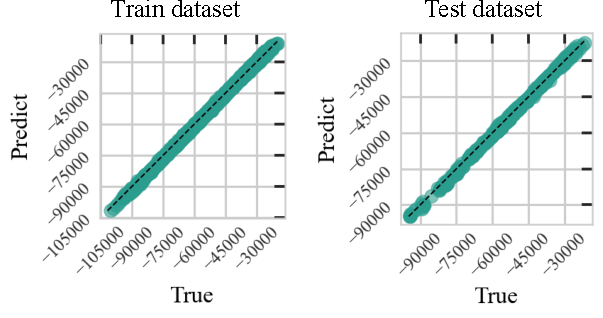
\includegraphics[width = 90mm]{main_images/figure-problem2-2.pdf}
        \caption{$\mathcal{G}^{(1)}$}
    \end{subfigure}%
    \vfill
    \begin{subfigure}[b]{\textwidth}
        \centering
        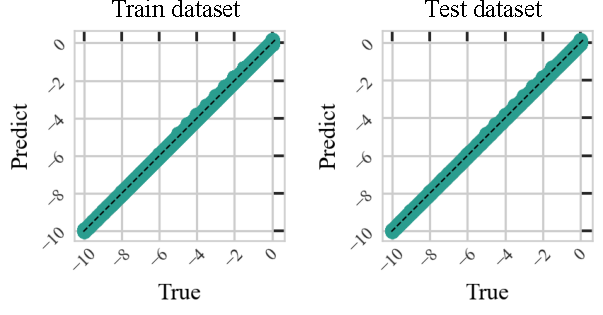
\includegraphics[width = 90mm]{main_images/figure-problem2-1.pdf}
        \caption{$\mathcal{G}^{(2)}$}
    \end{subfigure}%
    \vfill
    \begin{subfigure}[b]{\textwidth}
        \centering
        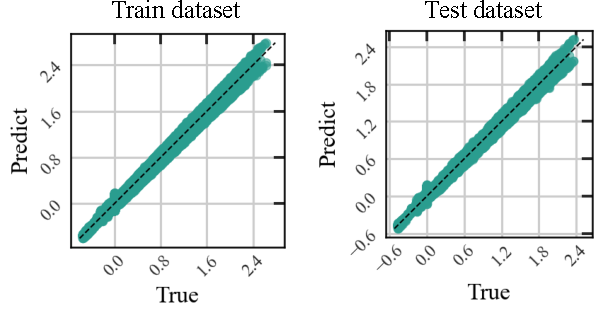
\includegraphics[width = 90mm]{main_images/figure-problem2-3.pdf}
        \caption{$\mathcal{G}^{(3)}$}
    \end{subfigure}%
    \caption{Triaxial metamodel performance: (a) Reaction force; (b) Axial deformation; (c) Radial deformation}
    \label{fig: triaxialperformance}
\end{figure}








\begin{figure}[htbp]
\centering
 \includegraphics[width=190mm]{main_images/figure-cornerplot.pdf}
 \caption{Corner plot for uncertain soil parameters}
 \label{fig: Cornerplot}
\end{figure}

% \begin{figure}[htbp]
% \centering
%  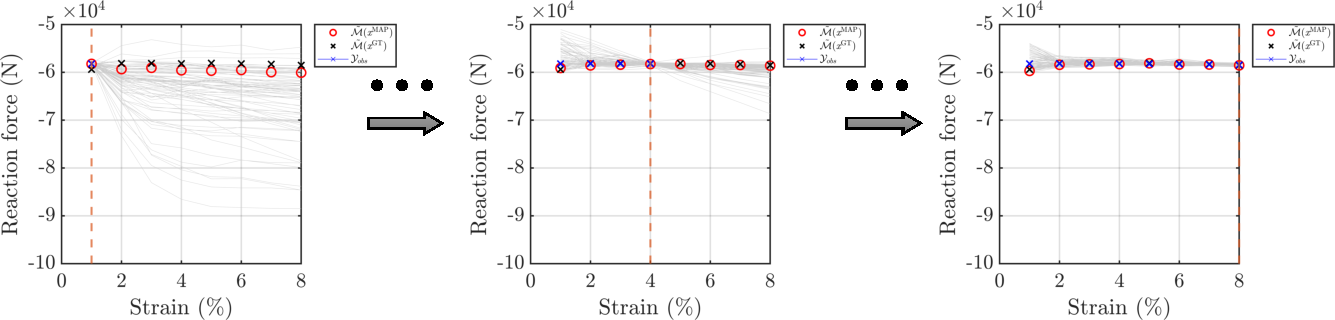
\includegraphics[width=140mm]{main_images/figure-UQ.pdf}
%  \caption{Uncertainty quantification process for reaction force}
%  \label{fig: UQ}
% \end{figure}
% \section{Additional remarks and limitations} \label{sec:limitation}




\section{Summary and Conclusions} \label{sec:conclusion}\noindent
This study introduced a simplified neural metamodel specifically designed to address the challenges of spatiotemporal, multi-field responses in geotechnical systems. By decoupling spatial and temporal learning while maintaining a unified latent representation, the proposed architecture links low-dimensional static soil parameters to complex, evolving outputs, including displacement fields, stress distributions and deformation vectors, within a single multi-output surrogate.

Through two benchmark problems, an offshore strip footing and a triaxial loading test, the metamodel demonstrated good predictive accuracy, robustness and efficiency. In the footing case, it captured both vector- and field-type responses across multiple loading stages with a test-set global normalised absolute error (GNAE) of about 2.3\%, while in the triaxial test the GNAE was about 1.3\%; For both examples, MAE and relative $L_2$ errors showed consistent trends for the investigated examples. Importantly, the metamodel was not only assessed in forward-prediction mode but also embedded in a sequential Bayesian calibration framework with multiple outputs, where it enabled efficient likelihood evaluations and led to a substantial reduction in parameter uncertainty as monitoring information accumulated.

The simplified architecture thus provides a practical balance between accuracy, computational efficiency and engineering applicability. Its modular, multi-output design facilitates extension to additional response quantities, heterogeneous soil conditions and more complex loading scenarios, and its compatibility with existing probabilistic tools makes it a promising surrogate for real-time prediction and uncertainty quantification in geotechnical practice. Future work may focus on enhancing generalisation to a wider range of constitutive models, incorporating spatial variability in ground conditions, mesh/geometry sensitivity and scaling the approach to large-scale infrastructure systems.
\section{Software and data availability}\label{sec: github}\noindent
FE model is running on \texttt{ABAQUS 2022} and all metamodel code related is trained based on \texttt{Python}, and MCMC is performed using \texttt{Matlab}. For interested readers, the dataset and related code will be found at \href{https://github.com/ningxin999/fullfield_spatiotemporal}{Github} to reproduce the figures.


\section{Declarations}\noindent
\textbf{Conflicts of interest}: The authors have no conflicts of interest to declare that are relevant to the content of this article.

\noindent\textbf{Ethics approval and consent to participate}: This is nonhuman subject research and waived the need for informed consent.

\noindent\textbf{Consent to participate/publish}: All authors contributed to the study conception and design. All authors read and approved the final
manuscript.


%\section{Acknowledgements}\noindent
The authors thank Dr. Randolf Altmeyer from the Department of Mathematics at Imperial College London for his assistance with the mathematical proofs.

%\input{acronym}


\clearpage
\newpage

\ifnum\classstyle=0
\printbibliography
\fi
\ifnum\classstyle=1
\printbibliography
\fi
\ifnum\classstyle=2
\printbibliography
\fi
\ifnum\classstyle=3
\printbibliography
\fi

\newpage
\appendix

\ifnum\online=0
%\input{09_Appendix}
\fi
\ifnum\online=1
%do nothing
\fi





\end{document}